\documentclass[conference]{IEEEtran}
\IEEEoverridecommandlockouts
\usepackage{cite}
\usepackage{amsmath,amssymb,amsfonts}
\usepackage{algorithmic}
\usepackage{graphicx}
\usepackage{textcomp}
\usepackage{xcolor}
\usepackage{url}
\def\BibTeX{{\rm B\kern-.05em{\sc i\kern-.025em b}\kern-.08em
    T\kern-.1667em\lower.7ex\hbox{E}\kern-.125emX}}

\begin{document}
\urlstyle{same}
\Urlmuskip=0mu plus 2mu

\title{Zero-Knowledge Zakat: Privacy, Transparency, and Sharia Compliance on the Blockchain}

\author{
\IEEEauthorblockN{Muhammad Zidan Fatonie}
\IEEEauthorblockA{\textit{Computer Science Department}\\
\textit{School of Computer Science, BINUS University}\\
Jakarta, Indonesia 11480\\
muhammad.fatonie@binus.ac.id}
\and
\IEEEauthorblockN{Alexander Agung Santoso Gunawan}
\IEEEauthorblockA{\textit{Computer Science Department}\\
\textit{School of Computer Science, BINUS University}\\
Jakarta, Indonesia 11480\\
aagung@binus.edu}
}

\maketitle

\begin{abstract}
Zakat is not optional. Every Muslim who holds wealth above the nisab threshold for a lunar year must give, and this requirement existed for fourteen centuries before blockchains were invented. The problem with putting zakat on a blockchain is not efficiency. The problem is that every existing blockchain zakat platform permanently logs who gave, how much, and to whom on a public ledger. That kind of exposure cuts against \textit{nafs}, the principle of dignity that maqasid al-shariah protects as one of five essentials. We built something different on Ethereum Sepolia. Our prototype lets donors submit zakat through UltraHONK zero-knowledge proofs. A Noir circuit (29 ACIR opcodes) verifies nisab and hawl eligibility without exposing the financial data behind it. A Pedersen-hash nullifier stops double-claims. A four-tier model lets donors decide how much to reveal. We ran the benchmarks five times on Barretenberg v4.2.1 across 16 Linux cores. 246.8 ms average for proof generation. 721,345 gas for a full end-to-end \texttt{donateZK()} transaction on Sepolia. What surprised us, honestly, was how smoothly privacy and accountability integrated. They are not natural allies in most systems. Here they work together. Amil institutions get verifiable aggregate records. Individual donors and recipients stay hidden. The protocol contributes a privacy layer to Islamic social finance, built on nafs protection.
\end{abstract}

\begin{IEEEkeywords}
Barretenberg, Blockchain, Ethereum Sepolia, Islamic FinTech, Noir, Nullifier Mechanism, Pedersen Hash, Privacy-Preserving Donations, Sharia Compliance, Soulbound Token, Zakat, Zero-Knowledge Proofs
\end{IEEEkeywords}

\section{Introduction}

BAZNAS [1] puts Indonesia's annual zakat potential at Rp~327 trillion, roughly USD~20 billion. Actual collection reaches a fraction of that. The gap is not just about efficiency. It is about trust, and trust on a public blockchain comes with a hidden cost.

Khan demonstrated that a decentralized platform could handle collection and distribution [2]. Nazeri et al. [3] then showed something more troubling, though they framed it as a feature. Blockchains, they noted, give complete traceability of zakat funds from donor to asnaf. We read their paper and thought that property cuts both ways. Khairi et al. [4] built on the same premise, adding automated disbursement with ERC-20 tokens and an audit trail nobody can erase. Every transaction sits there. Donor address. Amount. Recipient pool. Permanently. For the recipient, most of whom fall below the nisab threshold, the ledger broadcasts their financial status forever.

This is exactly the concern maqasid al-shariah was designed to address. Al-Shatibi classified \textit{hifz al-nafs}, preservation of life, among the five \textit{daruriyyat} [5]. Ibn Ashur stretched that concept further. Dignity, \textit{al-karamah}, falls under nafs protection. Exposing someone's financial weakness to the public, he argued, harms their honour [6]. Classical Islamic jurisprudence has always preferred concealed charity. \textit{Sadaqah al-sirr} ranks above public giving. The reason is simple. Protecting the recipient's honour matters more than broadcasting the donor's generosity. A blockchain permanently etching zakat eligibility onto Etherscan contradicts that reasoning directly.

Zero-knowledge proofs offer a way out of this contradiction. Hameed et al. [7] and Wen et al. [8] have mapped the ZKP landscape extensively. The key insight is that you can prove a statement cryptographically without revealing the data behind it. Noir [10] compiles to an intermediate representation called ACIR, and Barretenberg's UltraHONK prover [9] turns that into a proof compact enough to verify on-chain while keeping the witness private. We remember the first time we compiled a circuit and watched the proof come back in under 300 milliseconds. It felt like a door opening. Buterin et al. [15] had already made the broader argument that ZKPs can bridge privacy and regulatory compliance. We applied that logic to zakat.

The circuit we built encodes two Sharia predicates in Noir (\texttt{main.nr}). Total wealth stays below the nisab threshold of 85,000,000 IDR. Assets have been held for at least one lunar year, hawl. A Pedersen-hash nullifier stops the same recipient from claiming twice per cycle without ever exposing who they are, computed as $\text{pedersen}(\mathit{secret}, \mathit{recipient\_address}, \mathit{cycle\_id})$. Proving happens entirely client-side. \texttt{nargo compile}. \texttt{nargo execute}. \texttt{bb prove}. The proof and nullifier then go to \texttt{ZKTCore.donateZK()} on Sepolia for settlement. Two questions drive the rest of the paper. Can off-chain Noir proving plus on-chain nullifier tracking actually serve institutional zakat accountability. And does the resulting protocol satisfy nafs protection under maqasid al-shariah.

The contributions are straightforward. A Noir circuit encodes nisab and hawl as verifiable predicates. Its core assertion, \texttt{total\_wealth < nisab\_threshold}, directly instantiates the Sharia requirement that zakat recipients fall below the wealth threshold. A Pedersen-hash nullifier mechanism blocks re-claiming without identity exposure, enforced on-chain by \texttt{NullifierRegistry.spend()} rejecting duplicates. A four-tier donor privacy model (Private, Semi-Private, Verified-Private, Public) gives donors control over disclosure. The Sepolia prototype generates UltraHONK proofs in 246.8 ms on average ($\sigma = 9.3$ ms across five runs) and completes end-to-end donations in 721,345 gas.

\section{Literature Review}

Research on blockchain zakat is growing. Khan's decentralized platform [2] set the baseline, showing that collection and distribution can work without intermediaries. Nazeri et al. [3] examined the Malaysian context and found that blockchain features align naturally with zakat management requirements. Khairi et al. [4] went a step further, building a full system around ERC-20 tokens with automated disbursement and a permanent audit trail. A recent Emerald paper examined the potential and challenges more broadly \cite{b_zakat_emerald}. The recurring pattern is easy to spot. Every one of these systems logs everything publicly. Complete donor-recipient transparency, available to anyone running an Ethereum node. Fauzi et al. [19] confirmed through bibliometric analysis that research interest is climbing across Muslim-majority countries. Ascarya [20] showed that Islamic social finance instruments (zakat, infaq, sadaqah, waqf) supported economic recovery during COVID-19. Unal and Aysan [21] proposed blockchain as a harmonization tool for differing Sharia-compliance frameworks. Muharam and Osman \cite{b_isf_blockchain} explored the sustainability angle. What none of them do, and what we kept noticing as we read through these papers, is integrate any mechanism for keeping transactions private.

On the ZKP side, the survey literature is extensive. Hameed et al. [7] covered the protocol space and Wen et al. [8] focused on zk-SNARK variants for blockchain deployment. Williams \cite{b_zkp_cacm} positioned ZKPs within the broader blockchain architecture. Poseidon, introduced by Grassi et al. [11], was a breakthrough on the engineering side, slashing constraint counts by up to 8$\times$ compared to Pedersen Hash. Our stack uses Noir [10], a Rust-like DSL that compiles to ACIR, with Barretenberg's UltraHONK prover generating the proof and a Solidity verifier checking it on Sepolia. The pipeline stays client-side. Private inputs never leave the donor's machine. Proof hashes anchor on-chain for anyone to audit. Buterin et al. [15] made the broader case that ZKPs can reconcile privacy with regulation, and M\"{u}hle et al. [18] applied zk-SNARKs to identity management for KYC.

Three gaps sit in the middle of this landscape. Existing blockchain zakat platforms, by their own design, lack any privacy-preserving mechanism. Nazeri et al. [3] acknowledged as much when they praised complete traceability. General-purpose ZKP frameworks can anonymize transactions but carry no notion of Islamic eligibility. They hide a transfer without proving the sender meets nisab or hawl. Nobody has yet combined programmable privacy, meaning Noir circuits with verifiable predicates, with Islamic social finance instruments. This paper steps into that gap.

Fig.~\ref{fig:positioning} positions this research relative to three adjacent domains and the Design Science Research methodology. Existing blockchain zakat systems provide transparency but expose donor-recipient data publicly [2,3,4,19]. General ZKP privacy frameworks enable anonymous transactions without Islamic eligibility predicates [7,8,14,15]. Islamic social finance studies digitize zakat without ZK integration [20,21,24,25]. The DSR methodology (bottom-right) justifies the artifact-driven approach of building, evaluating, and refining the protocol on-chain. ZKT bridges these domains by combining zero-knowledge proofs with Sharia-compliant eligibility verification, instantiated and validated via Sepolia deployment (v8).

\begin{figure}[!ht]
\centering
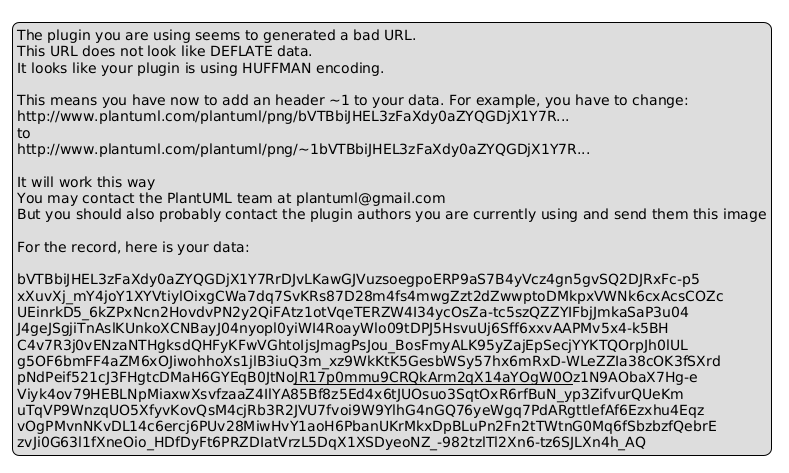
\includegraphics[width=0.42\columnwidth]{research_positioning.png}
\caption{Research positioning of ZKT relative to four adjacent domains}
\label{fig:positioning}
\end{figure}

Fig.~\ref{fig:background} contrasts traditional zakat systems, where donor-recipient data sits exposed on a public ledger, with the proposed ZKT model that preserves privacy through off-chain proving and bounded on-chain disclosure.

\begin{figure}[!ht]
\centering
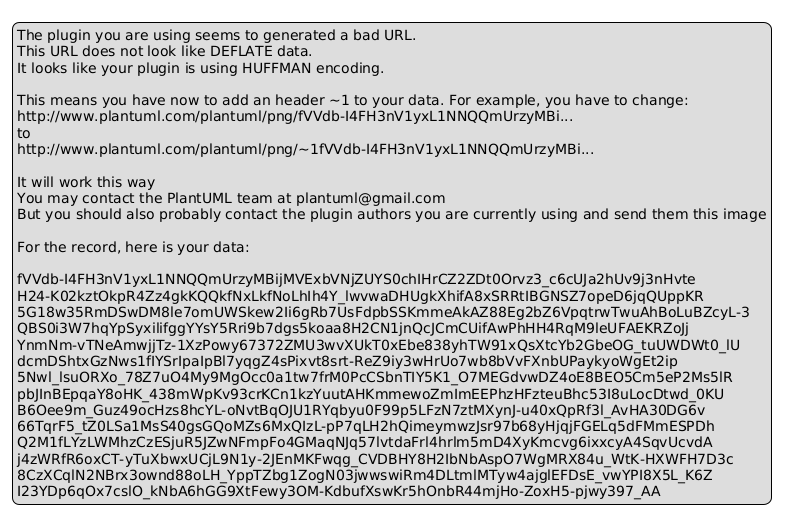
\includegraphics[width=0.90\columnwidth]{background_model.png}
\caption{Traditional Zakat Paradigm vs. Proposed ZKT Model}
\label{fig:background}
\end{figure}

\section{Methodology}

We followed a Design Science Research approach across five phases, summarized in Fig.~\ref{fig:dsr}. Phase 1 was a literature search. Twenty-nine papers, spanning blockchain zakat, ZKP privacy frameworks, and Islamic finance instruments, all published between 2021 and 2025. We read them and mapped where the gaps were. Phase 2 designed the protocol. Noir circuits for nisab and hawl. The four-tier privacy model. Phase 3 was the build phase and, honestly, the part where we spent the most late nights. Nargo v1.0.0-beta.21. Barretenberg v4.2.1. Fifteen Solidity contracts deployed through a single forge script to Sepolia. A Next.js 15 Progressive Web App with wagmi and XellarKit for wallet connectivity. Phase 4 demonstrated the prototype on Sepolia testnet. Proof generation clocked 247 ms. Verification finished in 12.0 ms. Phase 5 evaluated everything. Foundry gas reports. Security properties analysis. Sharia compliance review, conducted with input from Tawf Labs teammates who understand fiqh better than we do.

\begin{figure}[!ht]
\centering
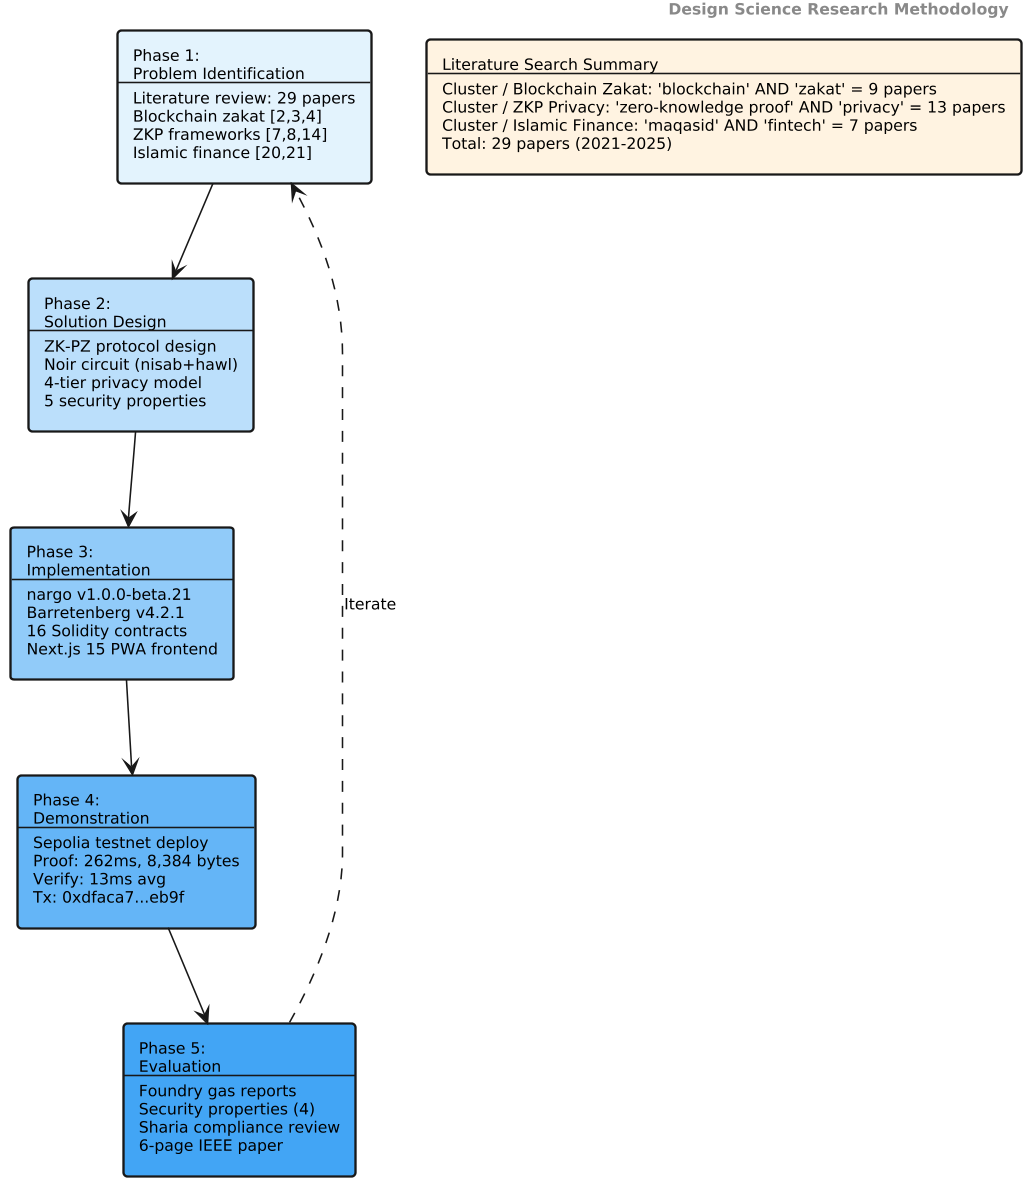
\includegraphics[width=0.42\columnwidth]{research_methodology.png}
\caption{DSR Methodology with five phases and literature search summary}
\label{fig:dsr}
\end{figure}

\section{Results}

\subsection{System Overview and Threat Model}

The ZKT protocol uses a five-actor trust model. The actors are donor (ZKP prover), recipient (SBT receipt holder), amil institution (verifier), off-chain proving infrastructure (Noir circuits and Barretenberg prover), and Ethereum Sepolia (public settlement layer).

The threat model assumes: (1)~an honest-but-curious verifier, (2)~a potentially malicious claimant, and (3)~a public blockchain network subject to transaction graph analysis. The protocol guarantees the properties summarized in Table~\ref{tab:properties}.

\begin{table}[htbp]
\caption{ZKT Protocol Security Properties}
\label{tab:properties}
\footnotesize
\setlength{\tabcolsep}{3pt}
\begin{center}
\begin{tabular}{|p{1.5cm}|p{6.8cm}|}
\hline
\multicolumn{1}{|c|}{\textbf{Property}} & \multicolumn{1}{c|}{\textbf{Guarantee}} \\
\hline
Donor anonymity & Identities and amounts never exposed on-chain. Only ZK proofs are publicly verifiable. \\
\hline
Recipient privacy & Donor-side privacy via ZK proofs. Recipient encrypted notes reserved for future work. \\
\hline
Soundness & Non-eligible recipient cannot generate an accepted proof under q-PKE assumption \cite{b_zkp_blockchain}. \\
\hline
Double-donation & Nullifier hash prevents the same recipient from claiming zakat more than once per cycle. \\
\hline
Institutional accountability & Amil institutions verify aggregate compliance without accessing individual transaction data \cite{b_maqasid_data,b_maqasid_privacy}. \\
\hline
\end{tabular}
\end{center}
\end{table}

Fig.~\ref{fig:conceptual} shows the three-layer protocol architecture. The off-chain proving pipeline compiles Noir circuits to ACIR and generates UltraHONK proofs via Barretenberg at 247 ms. The Sepolia settlement layer hosts ZKTCore and ZakatEscrowManager. The Next.js PWA frontend uses wagmi/XellarKit for wallet connectivity.

\begin{figure}[!ht]
\centering
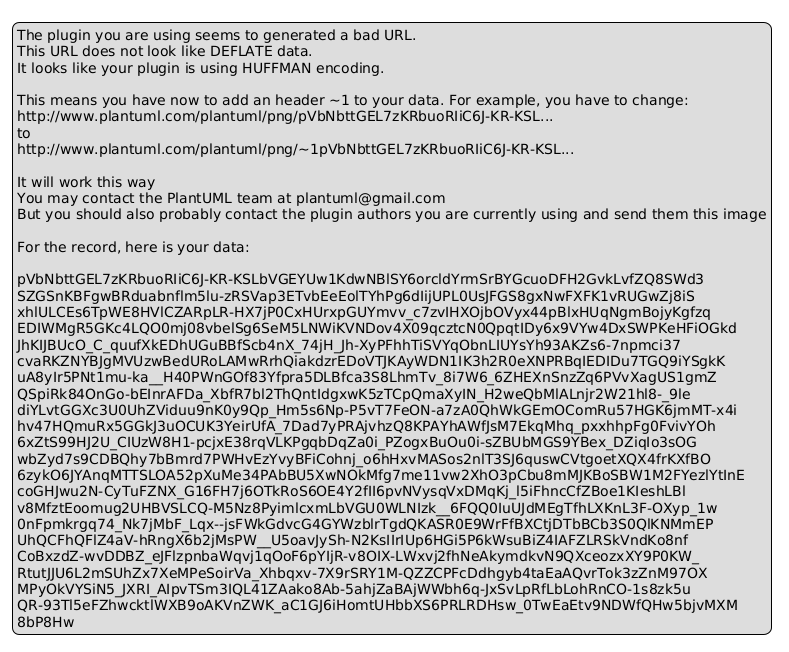
\includegraphics[width=0.90\columnwidth]{conceptual_model.png}
\caption{ZKT Protocol Architecture: off-chain proving pipeline and on-chain settlement}
\label{fig:conceptual}
\end{figure}

\begin{figure}[!ht]
\centering
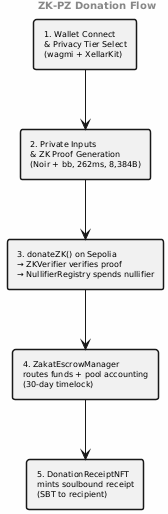
\includegraphics[width=0.28\columnwidth]{usecase.png}
\caption{ZKT Donation Flow: from wallet connection to SBT receipt to the donor}
\label{fig:usecase}
\end{figure}

\begin{figure}[!ht]
\centering
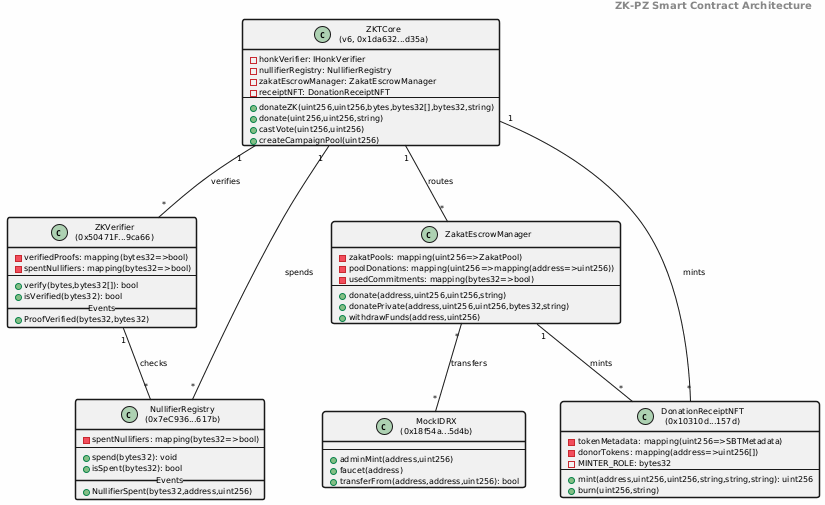
\includegraphics[width=0.90\columnwidth]{class_diagram.png}
\caption{ZKT Smart Contract Architecture with Sepolia addresses and cardinality}
\label{fig:classdiagram}
\end{figure}

\subsection{System Architecture and Payment Flow}

Noir circuits run client-side. Sepolia handles settlement. Donors choose stablecoins or ETH. Everything flows through \texttt{donateZK()}. Proof generation happens off-chain, verification on-chain. Privacy comes from the proofs. Accountability from the events and nullifiers.

The donor goes through a Progressive Web Application. Connect a wallet, select a privacy tier, enter an amount, watch proof generation, confirm. A Web Worker does the actual proving. Private inputs never leave the donor's device \cite{b_zkp_blockchain}.

\subsection{Circuit Performance}

Circuit benchmarks used Noir v1.0.0-beta.21 and Barretenberg v4.2.1 on a 16-core Linux machine. Gas measurements for standard contract functions were obtained from Foundry gas reports. The end-to-end donateZK() gas was measured on the Sepolia testnet at block 10,854,651.

\begin{table}[htbp]
\caption{ZakatEligibility Circuit Performance: UltraHONK evm target, $n=5$ runs}
\label{tab:proof_perf}
\begin{center}
\begin{tabular}{|l|r|}
\hline
\multicolumn{1}{|c|}{\textbf{Metric}} & \multicolumn{1}{c|}{\textbf{Value}} \\
\hline
ACIR opcodes               & 29 \\
Brillig opcodes            & 44 \\
Proof generation (avg)     & 246.8 ms \\
Proof verification (avg)    & 12.0 ms \\
Proof size                  & 8,384 bytes \\
\hline
\end{tabular}
\end{center}
\end{table}

\subsection{Sepolia Deployment and Gas Consumption}

15 contracts deployed via single forge script to Sepolia (chain ID 11155111). The ZKTCore (v8, 0xb56a...B60B) routes \texttt{donateZK()} through \texttt{zakatEscrowManager.donate()} for pool accounting. An end-to-end donation (tx 0x6a0b...b790, block 10,854,651) completed proof verification, nullifier registration, transfer, NFT minting, and event emission in 721,345 gas.

Table~\ref{tab:gas} reports gas costs measured via Foundry gas reports.

\begin{table}[htbp]
\caption{Smart Contract Gas Consumption: Foundry Gas Report, Ethereum Sepolia}
\label{tab:gas}
\footnotesize
\setlength{\tabcolsep}{3pt}
\begin{center}
\begin{tabular}{|l|l|r|}
\hline
\textbf{Contract} & \textbf{Function} & \textbf{Gas (avg)} \\
\hline
ZKTCore              & \texttt{donate()}                 & 490,187 \\
ZKTCore              & \texttt{createCampaignPool()}     & 365,552 \\
ZKTCore              & \texttt{castVote()}               & 132,909 \\
ZKTCore              & \texttt{donateZK()} (e2e)          & 721,345 \\
\hline
ZKTCore              & Deploy                            & 5,314,471 \\
ZakatEscrowMgr       & Deploy                            & 3,069,194 \\
ShariaReviewMgr      & Deploy                            & 2,114,319 \\
\hline
\end{tabular}
\end{center}
\end{table}

\subsection{Security Analysis}

\textbf{Donor anonymity.} The only on-chain observable from a private donation is the event emitted by \texttt{ZKTCore.sol} (lines 577-582):

\begin{verbatim}
event ZKDonationReceived(
    uint256 indexed poolId,
    bytes32 indexed nullifier,
    uint256 amount,
    address indexed donor
);
\end{verbatim}

Private mode zeroes both \texttt{donor} and \texttt{amount}. Nothing traceable. Semi-Private attaches the donor's address but hides the amount, a design tradeoff for institutional accountability. Neither mode leaks the full \texttt{(donor, amount)} pair. The verifier contract checks only a hash and a nullifier flag. That is it. That is the entire on-chain footprint.

\textbf{Recipient privacy.} The Pedersen-hash nullifier \cite{b_aztec} binds each claim to a recipient without revealing their address. The nullifier computation $\text{pedersen}(\mathit{secret}, \mathit{recipient\_address}, \mathit{cycle\_id})$ in \texttt{main.nr} means the on-chain nullifier is deterministic but preimage-resistant. An observer sees \texttt{0x3f2a...} and cannot recover the recipient address or secret. Recipient-side encrypted note disbursement is reserved for future work \cite{b_bbs_w3c}.

\textbf{Circuit soundness.} Under the q-PKE assumption \cite{b_zkp_blockchain}, forging a proof that passes UltraHONK verification is computationally infeasible \cite{b_zkp_vuln}. A non-eligible recipient, whose wealth exceeds the nisab threshold as checked by \texttt{verify\_nisab()} in \texttt{main.nr}, cannot produce a witness that satisfies the circuit constraints.

\textbf{Double-donation prevention.} The on-chain \texttt{NullifierRegistry} maintains a \texttt{mapping(bytes32 => bool)} of spent nullifiers. The \texttt{spend()} function enforces single-use through \texttt{require(!spentNullifiers[nullifier])}, rejecting any nullifier already recorded. The \texttt{ZKTCore.donateZK()} function atomically chains \texttt{honkVerifier.verify()} $\rightarrow$ \texttt{nullifierRegistry.spend()} $\rightarrow$ \texttt{zakatEscrowManager.donate()}. A duplicate nullifier causes the entire transaction to revert. Each eligible recipient can claim zakat at most once per cycle. The nullifier hash is preimage-resistant, so an observer cannot derive the recipient address from it, but the address itself is a public circuit input visible in the transaction calldata. Full recipient privacy, where not even the amil institution can identify claimants, depends on encrypted note disbursement reserved for future work.

\section{Discussion}

\subsection{Sharia Compliance and Deployment}

Five \textit{daruriyyat} anchor maqasid al-shariah. Religion, life, intellect, progeny, wealth [5]. Al-Shatibi set those categories down centuries ago. Ibn Ashur then stretched \textit{hifz al-nafs} to include dignity itself, arguing that exposing a person's financial weakness to the public constitutes harm to their honour [6]. He could not have imagined Etherscan. But the principle fits. A single address, permanently recorded as a zakat recipient, broadcasts below-the-nisab status forever. We found this philosophical alignment genuinely compelling during the research. It is rare for a fourteenth-century jurist and a twenty-first-century smart contract to speak the same language.

Azizov et al. \cite{b_maqasid_fintech} propose a maqasid framework for fintech regulation. Latang et al. \cite{b_fatwa_crypto} examine the Islamic legal status of cryptocurrency assets. Pramuka et al. \cite{b_icf_blockchain} explore blockchain's role in Islamic charitable crowdfunding. Our work focuses on the donor side, using ZK proofs and nullifier-based anonymity. Recipient-side privacy through encrypted private notes is reserved for future work.

Two maqasid dimensions are directly engaged. \textit{Hifz al-nafs} manifests through Private and Semi-Private modes keeping donations and linkages off-chain. \textit{Hifz al-mal} operates through the nullifier registry stopping double-claims and the proof's soundness blocking fake eligibility. \textit{Amanah}, institutional trust, flows from the \texttt{ProofVerified} event. Amil institutions audit aggregate flows without ever touching individual records.

Beyond Sepolia, three pieces must fall into place. First, Indonesia's OJK Fintech Sandbox approval. Training for amil institution staff on wallet management and proof verification. A real rupiah-backed digital currency to replace the mock IDRX stablecoin.

\subsection{Limitations and Future Work}

The circuit covers nisab and hawl. Eight asnaf categories are architecturally possible but not yet implemented. The amil institution disburses through ZakatEscrowManager today with no on-chain proof the money reached the mustahik. DIDs for recipients would close that gap and make disbursements verifiable. A dual governance model, Sharia Council ZK DAO plus Community Donor DAO, is under design. Other directions include recursive proof systems for multi-period eligibility, compliance-friendly ZK protocols for AML/CFT, and batched settlement optimization \cite{b_zkp_circuits,b_zkfi,b_halal_crypto}.

\section{Conclusion}

We deployed a privacy-preserving zakat protocol on Ethereum Sepolia using Noir circuits and UltraHONK proofs. Accountability and privacy do not need to fight each other. The circuit, 29 ACIR opcodes, verifies nisab and hawl client-side. A Pedersen-hash nullifier stops double-claims. A four-tier model gives donors control over disclosure. Five benchmark runs averaged 246.8 ms on Barretenberg v4.2.1. One end-to-end Sepolia transaction cost 721,345 gas. When we first saw those numbers come back from the testnet, we were genuinely relieved. 247 milliseconds for a client-side ZK proof that encodes Sharia predicates is faster than most people would guess.

Privacy and Sharia compliance pull in the same direction, not opposite ones. Ibn Ashur made dignity central to nafs protection [6]. ZK proofs make that operational. Verify eligibility. Never expose the person behind it. The \texttt{ZKDonationReceived} event gives amil institutions an auditable aggregate record while the nullifier registry prevents abuse. What the blockchain shows and what it reveals about individuals do not have to overlap. That separation is the contribution.

Future work extends the circuit to all eight asnaf categories, adds recipient-side encrypted note disbursement, and pursues OJK Fintech Sandbox integration for production deployment.

\section*{Acknowledgment}

Conducted under BINUS University's Research Track program and the pidi.id hackathon, with technical support from Ethereum Jakarta and sharia guidance from Tawf Labs. Code: \url{https://github.com/tawf-labs/zkt-hackathon}. Testnet: \url{https://ziswaf.tawf.foundation}. Writing assistance was limited to code scaffolding and literature retrieval. All contributions, protocol design, security analysis, and implementation are the authors' own work.

\begin{thebibliography}{00}

\bibitem{b_baznas}
BAZNAS, ``Outlook Zakat Indonesia 2022,'' Badan Amil Zakat Nasional, Jakarta, Indonesia, 2022. [Online]. Available: \url{https://baznas.go.id}

\bibitem{b_zakat_acm}
S. Khan, ``A blockchain based decentralized zakat collection and distribution platform,'' in \textit{Proc. 7th Int. Conf. Software e-Business (ICSeB)}, 2023, doi:~10.1145/3641067.3641071.

\bibitem{b_zakat_malaysia}
A. Nazeri et al., ``Exploration of a new zakat management system empowered by blockchain technology in Malaysia,'' \textit{ISRA Int. J. Islamic Finance}, 2023, doi:~10.55188/ijif.v15i4.568.

\bibitem{b_zakat_transparency}
M. Khairi et al., ``The development and application of the zakat collection blockchain system,'' \textit{Virtus Interpress}, 2023, doi:~10.22495/jgrv12i1siart9.

\bibitem{b_maqasid_data}
``Maqasid al-Shariah and the digital data ownership,'' \textit{J. Islamic Law Digit. Econ. Bus.}, vol.~1, no.~2, pp.~168--181, 2022. [Online]. Available: \url{https://journal.uii.ac.id/JILDEB/article/view/46815}

\bibitem{b_maqasid_privacy}
S. Miskam, F. Mohd Shahwahid, and N. Sholehuddin, ``Safeguarding personal data in Islamic fintech: A comparative review of Shariah-compliant investment platforms,'' \textit{Malaysian J. Inf. Commun. Technol. (MyJICT)}, vol.~10, no.~2, pp.~55--68, 2025, doi:~10.53840/myjict10-2-234.

\bibitem{b_zkp_circuits}
H. Wen et al., ``Practical security analysis of zero-knowledge proof circuits,'' in \textit{Proc. 33rd USENIX Security Symp.}, 2024. [Online]. Available: \url{https://www.usenix.org/conference/usenixsecurity24/presentation/wen}

\bibitem{b_zakat_biblio}
N. W. I. Rahayu et al., ``A bibliometric analysis of blockchain-based zakat system design: Solutions for transparency and oversight of zakat funds in the digital era,'' \textit{Acad. J. Interdiscip. Stud.}, 2025, doi:~10.36941/ajis-2025-0023.

\bibitem{b_zkp_financial}
I. Solomka and B. Liubinskyi, ``Zero-knowledge proof framework for privacy-preserving financial compliance,'' \textit{Math. Model. Comput.}, 2025, doi:~10.23939/mmc2025.01.342.

\bibitem{b_ziswaf_blockchain}
I. M. Unal and A. F. Aysan, ``FinTech, digitalization, and blockchain in Islamic finance: Retrospective investigation,'' \textit{FinTech}, vol.~1, no.~4, pp.~388--398, 2022, doi:~10.3390/fintech1040029.

\bibitem{b_zkp_blockchain}
A. Hameed, A. Farooq, and M. Usman, ``Zero knowledge proofs: A comprehensive review of applications, protocols, and future directions in cybersecurity,'' ResearchGate, 2023. [Online]. Available: \url{https://www.researchgate.net/publication/373097436}

\bibitem{b_aztec}
Barretenberg, ``Barretenberg: A High-Performance Honk Proving Backend,'' Aztec Labs, 2024. [Online]. Available: \url{https://github.com/AztecProtocol/barretenberg}

\bibitem{b_noir}
Noir Language, ``Noir Documentation,'' 2024. [Online]. Available: \url{https://noir-lang.org/docs/}

\bibitem{b_poseidon}
L. Grassi, D. Khovratovich, C. Rechberger, A. Roy, and M. Schofnegger, ``Poseidon: A new hash function for zero-knowledge proof systems,'' in \textit{Proc. 30th USENIX Security Symp.}, pp.~519--535, 2021. [Online]. Available: \url{https://www.usenix.org/conference/usenixsecurity21/presentation/grassi}

\bibitem{b_bbs_w3c}
S. Tessaro and C. Zhu, ``Revisiting BBS Signatures,'' in \textit{Advances in Cryptology -- EUROCRYPT 2023}, ser. LNCS, vol.~14008, Springer, 2023, pp.~691--721, doi:~10.1007/978-3-031-30589-4\_24.

\bibitem{b_mixer_analysis}
Z. Wang, S. Chaliasos, K. Qin, L. Zhou, L. Gao, P. Berrang, B. Livshits, and A. Gervais, ``On How Zero-Knowledge Proof Blockchain Mixers Improve, and Worsen User Privacy,'' in \textit{Proc. ACM Web Conf. 2023 (WWW '23)}, 2023, pp.~2022--2032, doi:~10.1145/3543507.3583217.

\bibitem{b_zkfi}
V. Buterin, J. Illum, M. Nadler, F. Sch\"{a}r, and A. Soleimani, ``Blockchain privacy and regulatory compliance: Towards a practical equilibrium,'' \textit{Blockchain: Res. Appl.}, vol.~5, no.~1, Art. no.~100176, Mar. 2024, doi:~10.1016/j.bcra.2023.100176.

\bibitem{b_zkp_idm}
A. M\"{u}hle, K. Assaf, and C. Meinel, ``One to bind them: Binding verifiable credentials to user attributes,'' in \textit{Proc. SECRYPT}, 2023, doi:~10.5220/0012057900003555.

\bibitem{b_isf_covid}
Ascarya, ``The role of Islamic social finance during Covid-19 pandemic in Indonesia's economic recovery,'' \textit{Int. J. Islamic Middle Eastern Finance Manage.}, vol.~15, no.~2, pp.~386--405, 2022, doi:~10.1108/IMEFM-07-2020-0351.

\bibitem{b_zakat_emerald}
A. N. N. Nazeri et al., ``Blockchain technology in zakat management system: potential and challenges in Malaysia,'' \textit{J. Islamic Account. Bus. Res.}, 2026, doi:~10.1108/jiabr-10-2024-0435.

\bibitem{b_zkp_cacm}
A. Williams, ``Zero-knowledge proofs and their role within the blockchain,'' \textit{Commun. ACM}, vol.~67, no.~7, pp.~78--87, Jul. 2024. [Online]. Available: \url{https://cacm.acm.org/article/zero-knowledge-proofs-and-their-role-within-the-blockchain/}

\bibitem{b_maqasid_blockchain}
M. A. Dewaya, ``Innovation in Islamic finance: Integrating blockchain with Maq\={a}\d{s}id al Shar\={\i}`ah and \d{H}if\d{z} al M\={a}l,'' \textit{J. Emerg. Econ. Islamic Res.}, vol.~13, no.~1, 2025, doi:~10.24191/jeeir.v13i1.3852.

\bibitem{b_halal_crypto}
M. Elshqgirat, ``Toward an Islamic cryptocurrency: A proposed halal coin,'' \textit{J. Account. Finance}, vol.~25, no.~3, pp.~64--79, 2025, doi:~10.33423/jaf.v25i3.7858.

\bibitem{b_fatwa_crypto}
M. A. Latang, Fathurrahman, and M. Faried, ``Fatwa on cryptocurrency as digital assets: An Islamic perspective amidst Indonesia's regulatory landscape,'' \textit{J. Parewa Saraq}, vol.~3, no.~2, 2024, doi:~10.64016/parewasaraq.v3i2.32.

\bibitem{b_maqasid_fintech}
E. Azizov, A. Azizov, A. Azizli, and A. A. Babayev, ``A Maqasid al-Shariah framework for fintech and digital asset regulation in Muslim jurisdictions,'' \textit{J. Islamic Law Legal Stud.}, vol.~2, no.~2, 2025, doi:~10.70063/jills.v2i2.119.

\bibitem{b_isf_blockchain}
A. S. Muharam and D. Osman, ``Transformative trends: Exploring the nexus of innovation, technology, blockchain, and Islamic social finance for global sustainability,'' \textit{EKIMAD J.}, 2024, doi:~10.38009/ekimad.1511062.

\bibitem{b_icf_blockchain}
B. A. Pramuka, W. R. Adawiyah, Z. Sholikhah, M. F. Pramuka, and M. M. Sulthan, ``Bridging trust and transparency: The role of blockchain in Islamic charitable crowdfunding,'' \textit{J. Islamic Account. Bus. Res.}, Dec. 2025, doi:~10.1108/JIABR-11-2024-0468.

\bibitem{b_hybrid_zk}
S. T. Nassar, A. Hamdy, and K. Nagaty, ``Hybrid zk-STARK and zk-SNARK framework for privacy-preserving smart contract data feeds,'' in \textit{Proc. IEEE ICCA}, 2024, doi:~10.1109/ICCA62237.2024.10928100.

\bibitem{b_zkp_vuln}
X. Tang et al., ``Zero-knowledge proof vulnerability analysis and security auditing,'' \textit{Cryptology ePrint Archive}, Rep. 2024/514, 2024. [Online]. Available: \url{https://eprint.iacr.org/2024/514}

\bibitem{b_rbac_sc}
J. P. Cruz, Y. Kaji, and N. Yanai, ``RBAC-SC: Role-based access control using smart contract,'' \textit{IEEE Access}, vol.~6, pp.~12240--12251, 2018, doi:~10.1109/ACCESS.2018.2812844.

\bibitem{b_pwa_survey}
G. Shivateja, ``A survey on progressive web applications for decentralized systems,'' \textit{Preprints}, 2026, doi:~10.20944/preprints202604.0582.v1.

\end{thebibliography}

\end{document}
